\documentclass[twoside]{book}

% Packages required by doxygen
\usepackage{fixltx2e}
\usepackage{calc}
\usepackage{doxygen}
\usepackage[export]{adjustbox} % also loads graphicx
\usepackage{graphicx}
\usepackage[utf8]{inputenc}
\usepackage{makeidx}
\usepackage{multicol}
\usepackage{multirow}
\PassOptionsToPackage{warn}{textcomp}
\usepackage{textcomp}
\usepackage[nointegrals]{wasysym}
\usepackage[table]{xcolor}

% Font selection
\usepackage[T1]{fontenc}
\usepackage[scaled=.90]{helvet}
\usepackage{courier}
\usepackage{amssymb}
\usepackage{sectsty}
\renewcommand{\familydefault}{\sfdefault}
\allsectionsfont{%
  \fontseries{bc}\selectfont%
  \color{darkgray}%
}
\renewcommand{\DoxyLabelFont}{%
  \fontseries{bc}\selectfont%
  \color{darkgray}%
}
\newcommand{\+}{\discretionary{\mbox{\scriptsize$\hookleftarrow$}}{}{}}

% Page & text layout
\usepackage{geometry}
\geometry{%
  a4paper,%
  top=2.5cm,%
  bottom=2.5cm,%
  left=2.5cm,%
  right=2.5cm%
}
\tolerance=750
\hfuzz=15pt
\hbadness=750
\setlength{\emergencystretch}{15pt}
\setlength{\parindent}{0cm}
\setlength{\parskip}{3ex plus 2ex minus 2ex}
\makeatletter
\renewcommand{\paragraph}{%
  \@startsection{paragraph}{4}{0ex}{-1.0ex}{1.0ex}{%
    \normalfont\normalsize\bfseries\SS@parafont%
  }%
}
\renewcommand{\subparagraph}{%
  \@startsection{subparagraph}{5}{0ex}{-1.0ex}{1.0ex}{%
    \normalfont\normalsize\bfseries\SS@subparafont%
  }%
}
\makeatother

% Headers & footers
\usepackage{fancyhdr}
\pagestyle{fancyplain}
\fancyhead[LE]{\fancyplain{}{\bfseries\thepage}}
\fancyhead[CE]{\fancyplain{}{}}
\fancyhead[RE]{\fancyplain{}{\bfseries\leftmark}}
\fancyhead[LO]{\fancyplain{}{\bfseries\rightmark}}
\fancyhead[CO]{\fancyplain{}{}}
\fancyhead[RO]{\fancyplain{}{\bfseries\thepage}}
\fancyfoot[LE]{\fancyplain{}{}}
\fancyfoot[CE]{\fancyplain{}{}}
\fancyfoot[RE]{\fancyplain{}{\bfseries\scriptsize Generated by Doxygen }}
\fancyfoot[LO]{\fancyplain{}{\bfseries\scriptsize Generated by Doxygen }}
\fancyfoot[CO]{\fancyplain{}{}}
\fancyfoot[RO]{\fancyplain{}{}}
\renewcommand{\footrulewidth}{0.4pt}
\renewcommand{\chaptermark}[1]{%
  \markboth{#1}{}%
}
\renewcommand{\sectionmark}[1]{%
  \markright{\thesection\ #1}%
}

% Indices & bibliography
\usepackage{natbib}
\usepackage[titles]{tocloft}
\setcounter{tocdepth}{3}
\setcounter{secnumdepth}{5}
\makeindex

% Hyperlinks (required, but should be loaded last)
\usepackage{ifpdf}
\ifpdf
  \usepackage[pdftex,pagebackref=true]{hyperref}
\else
  \usepackage[ps2pdf,pagebackref=true]{hyperref}
\fi
\hypersetup{%
  colorlinks=true,%
  linkcolor=blue,%
  citecolor=blue,%
  unicode%
}

% Custom commands
\newcommand{\clearemptydoublepage}{%
  \newpage{\pagestyle{empty}\cleardoublepage}%
}

\usepackage{caption}
\captionsetup{labelsep=space,justification=centering,font={bf},singlelinecheck=off,skip=4pt,position=top}

%===== C O N T E N T S =====

\begin{document}

% Titlepage & ToC
\hypersetup{pageanchor=false,
             bookmarksnumbered=true,
             pdfencoding=unicode
            }
\pagenumbering{alph}
\begin{titlepage}
\vspace*{7cm}
\begin{center}%
{\Large My Project }\\
\vspace*{1cm}
{\large Generated by Doxygen 1.8.13}\\
\end{center}
\end{titlepage}
\clearemptydoublepage
\pagenumbering{roman}
\tableofcontents
\clearemptydoublepage
\pagenumbering{arabic}
\hypersetup{pageanchor=true}

%--- Begin generated contents ---
\chapter{Hierarchical Index}
\section{Class Hierarchy}
This inheritance list is sorted roughly, but not completely, alphabetically\+:\begin{DoxyCompactList}
\item \contentsline{section}{Animaux}{\pageref{classAnimaux}}{}
\begin{DoxyCompactList}
\item \contentsline{section}{Animaux\+De\+Denis}{\pageref{classAnimauxDeDenis}}{}
\item \contentsline{section}{Animaux\+De\+Florent}{\pageref{classAnimauxDeFlorent}}{}
\end{DoxyCompactList}
\end{DoxyCompactList}

\chapter{Class Index}
\section{Class List}
Here are the classes, structs, unions and interfaces with brief descriptions\+:\begin{DoxyCompactList}
\item\contentsline{section}{\hyperlink{classAnimaux}{Animaux} }{\pageref{classAnimaux}}{}
\item\contentsline{section}{\hyperlink{classAnimauxDeDenis}{Animaux\+De\+Denis} }{\pageref{classAnimauxDeDenis}}{}
\item\contentsline{section}{\hyperlink{classAnimauxDeFlorent}{Animaux\+De\+Florent} }{\pageref{classAnimauxDeFlorent}}{}
\end{DoxyCompactList}

\chapter{Class Documentation}
\hypertarget{classAnimaux}{}\section{Animaux Class Reference}
\label{classAnimaux}\index{Animaux@{Animaux}}


Inheritance diagram for Animaux\+:
\nopagebreak
\begin{figure}[H]
\begin{center}
\leavevmode
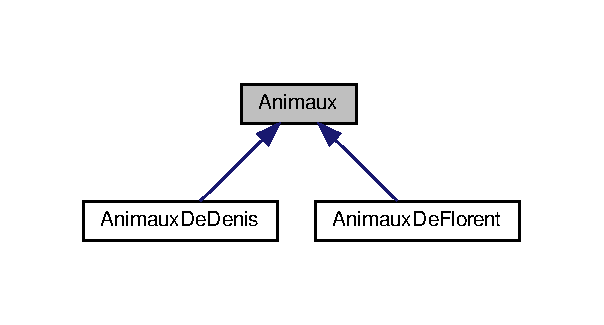
\includegraphics[width=290pt]{classAnimaux__inherit__graph}
\end{center}
\end{figure}
\subsection*{Public Member Functions}
\begin{DoxyCompactItemize}
\item 
\mbox{\Hypertarget{classAnimaux_a773b9db3c6694b6386bf90d02df1cb30}\label{classAnimaux_a773b9db3c6694b6386bf90d02df1cb30}} 
{\bfseries Animaux} (string nom, int PV, int puissance)
\item 
\mbox{\Hypertarget{classAnimaux_a5d0a273721dbea9d5fde827ca32ae120}\label{classAnimaux_a5d0a273721dbea9d5fde827ca32ae120}} 
void {\bfseries attaque} (\hyperlink{classAnimaux}{Animaux} $\ast$target)
\item 
\mbox{\Hypertarget{classAnimaux_a9f1774b7fd8859d3fc1bcdd1ec962543}\label{classAnimaux_a9f1774b7fd8859d3fc1bcdd1ec962543}} 
virtual void {\bfseries attaque\+\_\+de\+\_\+la\+\_\+mort} (\hyperlink{classAnimaux}{Animaux} $\ast$target)=0
\item 
\mbox{\Hypertarget{classAnimaux_a3a81004be25acde17fef26e3424f91cc}\label{classAnimaux_a3a81004be25acde17fef26e3424f91cc}} 
virtual void {\bfseries attaque\+\_\+faible} (\hyperlink{classAnimaux}{Animaux} $\ast$target)=0
\end{DoxyCompactItemize}
\subsection*{Public Attributes}
\begin{DoxyCompactItemize}
\item 
\mbox{\Hypertarget{classAnimaux_aaa578d600c1a221c198256ffc409c047}\label{classAnimaux_aaa578d600c1a221c198256ffc409c047}} 
string {\bfseries nom}
\item 
\mbox{\Hypertarget{classAnimaux_ab44bc431f44a297eddc8e66bfc2a0f1d}\label{classAnimaux_ab44bc431f44a297eddc8e66bfc2a0f1d}} 
int {\bfseries PV}
\item 
\mbox{\Hypertarget{classAnimaux_a3a12242e4112a67c50fd43d9c36e5d28}\label{classAnimaux_a3a12242e4112a67c50fd43d9c36e5d28}} 
int {\bfseries puissance}
\end{DoxyCompactItemize}


The documentation for this class was generated from the following files\+:\begin{DoxyCompactItemize}
\item 
animaux.\+h\item 
animaux.\+cpp\end{DoxyCompactItemize}

\hypertarget{classAnimauxDeDenis}{}\section{Animaux\+De\+Denis Class Reference}
\label{classAnimauxDeDenis}\index{Animaux\+De\+Denis@{Animaux\+De\+Denis}}


Inheritance diagram for Animaux\+De\+Denis\+:
\nopagebreak
\begin{figure}[H]
\begin{center}
\leavevmode
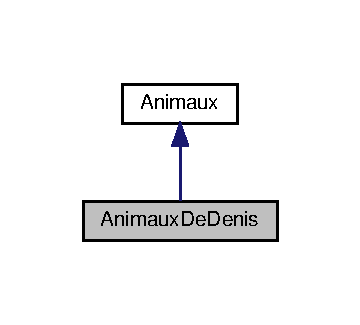
\includegraphics[width=173pt]{classAnimauxDeDenis__inherit__graph}
\end{center}
\end{figure}


Collaboration diagram for Animaux\+De\+Denis\+:
\nopagebreak
\begin{figure}[H]
\begin{center}
\leavevmode
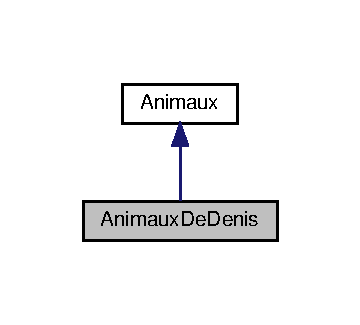
\includegraphics[width=173pt]{classAnimauxDeDenis__coll__graph}
\end{center}
\end{figure}
\subsection*{Public Member Functions}
\begin{DoxyCompactItemize}
\item 
\mbox{\Hypertarget{classAnimauxDeDenis_a56245bce148da0875882b24da0ee43c7}\label{classAnimauxDeDenis_a56245bce148da0875882b24da0ee43c7}} 
{\bfseries Animaux\+De\+Denis} (string nom, int PV, int puissance, int magie)
\item 
\mbox{\Hypertarget{classAnimauxDeDenis_ad0bf041f421e1dfdcda5fe70e5c2074f}\label{classAnimauxDeDenis_ad0bf041f421e1dfdcda5fe70e5c2074f}} 
void {\bfseries attaque\+\_\+de\+\_\+la\+\_\+mort} (\hyperlink{classAnimaux}{Animaux} $\ast$target)
\item 
\mbox{\Hypertarget{classAnimauxDeDenis_a3b50240079636df486a11e942f8fe39d}\label{classAnimauxDeDenis_a3b50240079636df486a11e942f8fe39d}} 
void {\bfseries attaque\+\_\+faible} (\hyperlink{classAnimaux}{Animaux} $\ast$target)
\end{DoxyCompactItemize}
\subsection*{Public Attributes}
\begin{DoxyCompactItemize}
\item 
\mbox{\Hypertarget{classAnimauxDeDenis_a42f9bd30c663ce2227ae4df0aa36914b}\label{classAnimauxDeDenis_a42f9bd30c663ce2227ae4df0aa36914b}} 
int {\bfseries magie}
\end{DoxyCompactItemize}


The documentation for this class was generated from the following files\+:\begin{DoxyCompactItemize}
\item 
denis.\+h\item 
denis.\+cpp\end{DoxyCompactItemize}

\hypertarget{classAnimauxDeFlorent}{}\section{Animaux\+De\+Florent Class Reference}
\label{classAnimauxDeFlorent}\index{Animaux\+De\+Florent@{Animaux\+De\+Florent}}


Inheritance diagram for Animaux\+De\+Florent\+:
\nopagebreak
\begin{figure}[H]
\begin{center}
\leavevmode
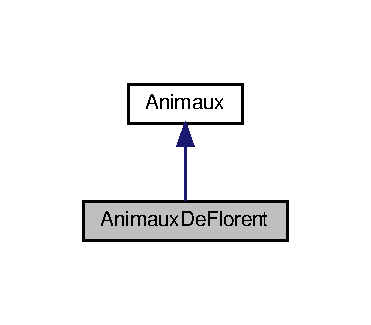
\includegraphics[width=178pt]{classAnimauxDeFlorent__inherit__graph}
\end{center}
\end{figure}


Collaboration diagram for Animaux\+De\+Florent\+:
\nopagebreak
\begin{figure}[H]
\begin{center}
\leavevmode
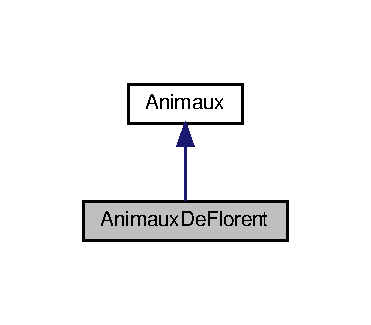
\includegraphics[width=178pt]{classAnimauxDeFlorent__coll__graph}
\end{center}
\end{figure}
\subsection*{Public Member Functions}
\begin{DoxyCompactItemize}
\item 
\mbox{\Hypertarget{classAnimauxDeFlorent_ab9388f02bac71adb781ca9d18a63fb79}\label{classAnimauxDeFlorent_ab9388f02bac71adb781ca9d18a63fb79}} 
{\bfseries Animaux\+De\+Florent} (string nom, int PV, int puissance, int arme)
\item 
\mbox{\Hypertarget{classAnimauxDeFlorent_ae63f1ba7abd46afb2fa8782cd088ece6}\label{classAnimauxDeFlorent_ae63f1ba7abd46afb2fa8782cd088ece6}} 
void {\bfseries attaque\+\_\+de\+\_\+la\+\_\+mort} (\hyperlink{classAnimaux}{Animaux} $\ast$target)
\item 
\mbox{\Hypertarget{classAnimauxDeFlorent_a76903cdaaac488dced777b9863f78c55}\label{classAnimauxDeFlorent_a76903cdaaac488dced777b9863f78c55}} 
void {\bfseries attaque\+\_\+faible} (\hyperlink{classAnimaux}{Animaux} $\ast$target)
\end{DoxyCompactItemize}
\subsection*{Public Attributes}
\begin{DoxyCompactItemize}
\item 
\mbox{\Hypertarget{classAnimauxDeFlorent_af04cb1ffb17ba177f70ee756cc09c1d7}\label{classAnimauxDeFlorent_af04cb1ffb17ba177f70ee756cc09c1d7}} 
int {\bfseries arme}
\end{DoxyCompactItemize}


The documentation for this class was generated from the following files\+:\begin{DoxyCompactItemize}
\item 
florent.\+h\item 
florent.\+cpp\end{DoxyCompactItemize}

%--- End generated contents ---

% Index
\backmatter
\newpage
\phantomsection
\clearemptydoublepage
\addcontentsline{toc}{chapter}{Index}
\printindex

\end{document}
